\graphicspath{{lit_study/fig/}}

\chapter{Literature study}
\label{chap:lit_study}

\section{Unknown suspended payloads}

    \paragraph
    Figure~\ref{fig:real_suspended_payload_example} shows an example of a practical use case of a multirotor with a suspended payload.
    Items are placed in a water proof bag and transported by the multirotor to a place of need.
    Note that the multirotor does not know the dynamics of the payload before flight, 
    because the items may change depending on the need in the specific situation. 
    The shape and mass of the loaded items will have an effect on swing of the payload, 
    and the control system should be able to fly well despite the altered flight dynamics.

    \begin{figure}[htb]
        \centering
        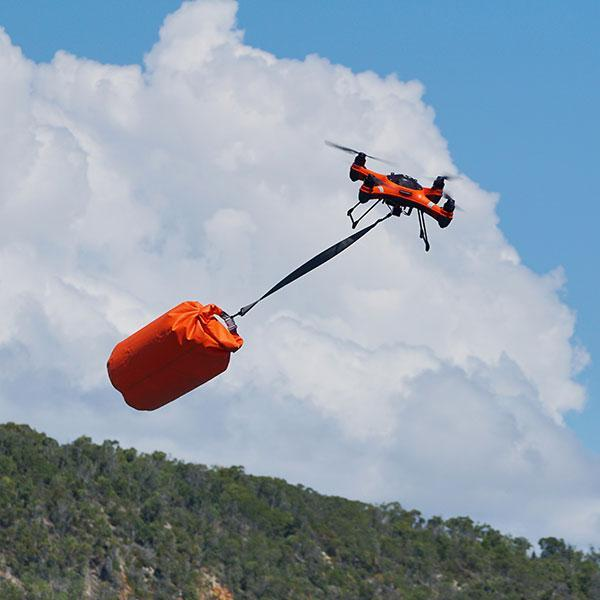
\includegraphics[width=0.45\linewidth]{real_suspended_payload_example.jpg}            
        \caption{A practical suspended payload used for search and rescue missions \cite{CompareCommander2020}}
        \label{fig:real_suspended_payload_example}
    \end{figure}

\section{System Identification}
\section{Control systems}
\section{System Design}
Blok diagram
komponente



